\documentclass[12pt]{article}
\usepackage[margin=0.8in]{geometry}
\usepackage{listings}
\usepackage{xcolor}
\usepackage{graphicx}
\usepackage{caption}
\usepackage{hyperref}

\graphicspath{ {./screenshots/} }

\hypersetup{
    bookmarksnumbered=true,
    colorlinks=true,
    linkcolor=blue,
    filecolor=magenta,      
    urlcolor=cyan,
    pdftitle={Contents},
    pdfpagemode=FullScreen,
}

\definecolor{codegreen}{rgb}{0,0.6,0}
\definecolor{codegray}{rgb}{0.5,0.5,0.5}
\definecolor{codepurple}{rgb}{0.58,0,0.82}
\definecolor{backcolour}{rgb}{0.95,0.95,0.92}

\lstdefinestyle{mystyle}{
    backgroundcolor=\color{backcolour},   
    commentstyle=\color{codegreen},
    keywordstyle=\color{magenta},
    numberstyle=\tiny\color{codegray},
    stringstyle=\color{codepurple},
    basicstyle=\ttfamily\footnotesize,
    breakatwhitespace=false,         
    breaklines=true,                 
    captionpos=b,                    
    keepspaces=true,                 
    numbers=left,                    
    numbersep=5pt,                  
    showspaces=false,                
    showstringspaces=false,
    showtabs=false,                  
    tabsize=2
}

\lstset{
  frame=single,
  style=mystyle
}

\renewcommand{\lstlistingname}{Code}% Listing -> Code
\renewcommand{\lstlistlistingname}{List of \lstlistingname s}% List of Listings -> List of Code

\captionsetup[lstlisting]{font=tt}

\title{CDE204 Matlab report}
\author{Nguyen Tien Dat}
\date{March 2023}

\begin{document}
\maketitle
\newpage
\tableofcontents
\addcontentsline{toc}{section}{Contents} % add this line

\lstlistoflistings
\addcontentsline{toc}{section}{\lstlistlistingname} % add this line

\listoffigures
\addcontentsline{toc}{section}{\listfigurename} % add this line


\newpage
\section{QAM modulation over AQGN channel}

\subsection{Use bertool}
\begin{figure}[ht]
    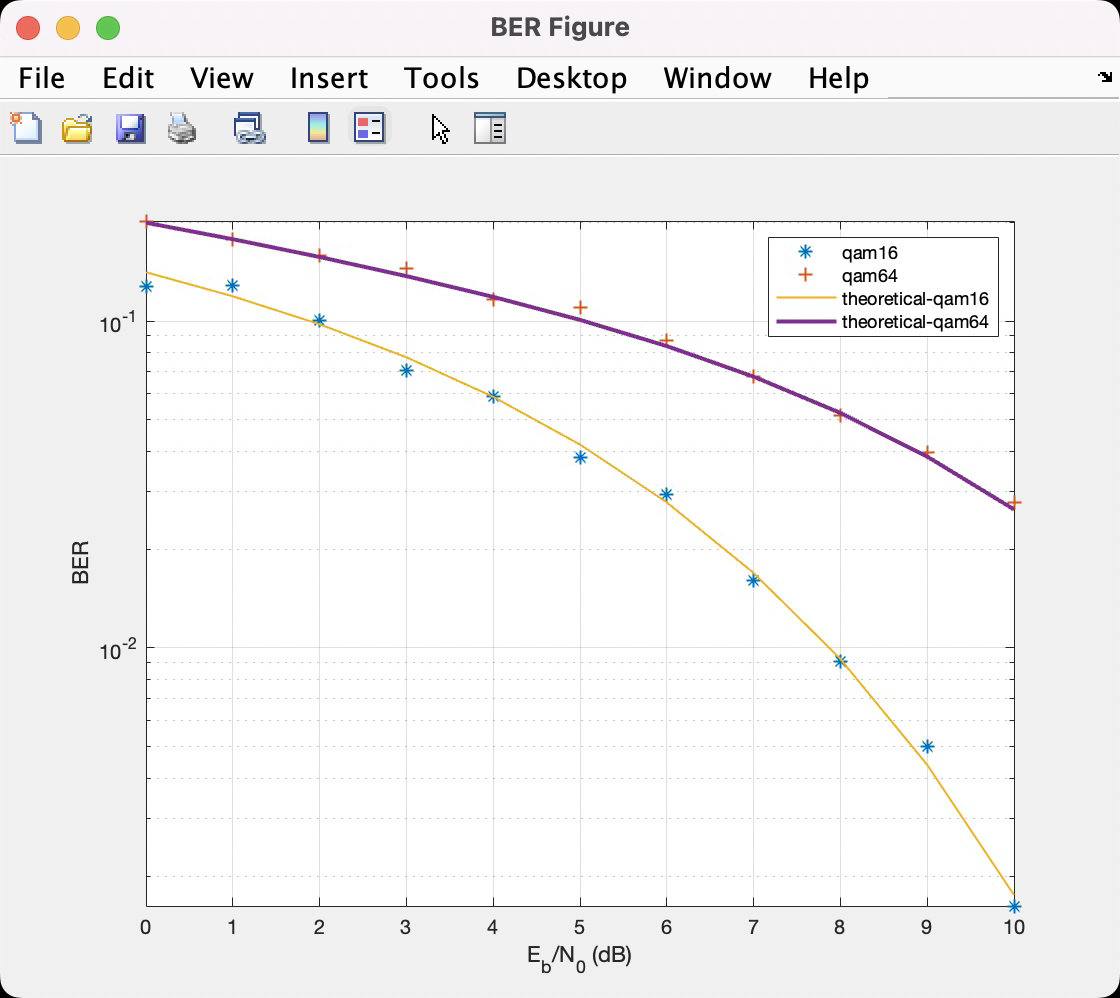
\includegraphics[width=\textwidth]{bertool}
    \caption{BER drawing using bertool}
\end{figure}

I realized that when use bertool, the simulation should be faster than code the
by myself. But there two many mouse action that I am not be a fan of. So here after,
I code the scenarios myself to reduce the time taken.

\subsection{Self made script}

\lstinputlisting[language=Matlab, caption={qam\_M.m}]{./matlab/qam_M.m}

\lstinputlisting[language=Matlab, caption={test\_qam\_M.m}]{./matlab/test_qam_M.m}

\begin{figure}[ht]
    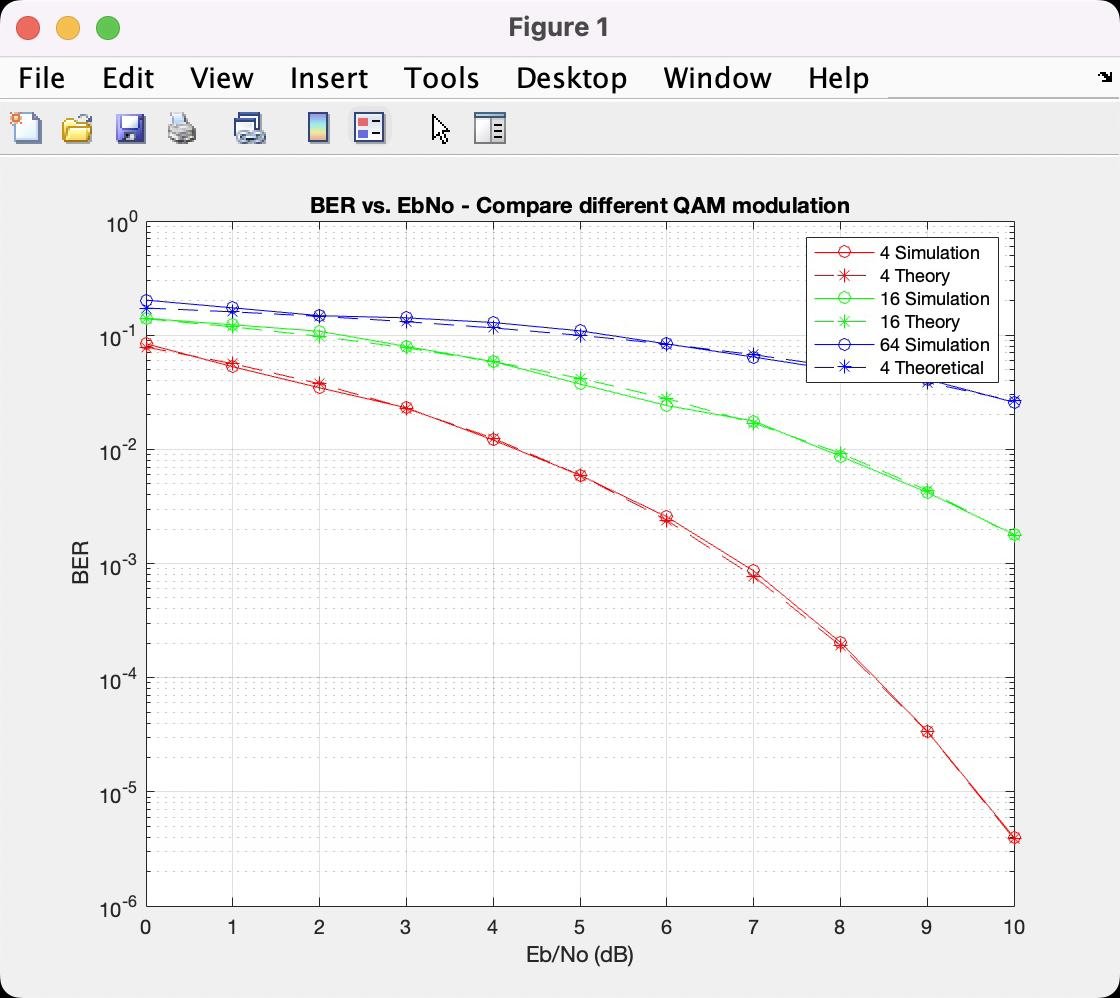
\includegraphics[width=\textwidth]{qam}
    \caption{BER Different QAM level}
\end{figure}

\section{Compare BER with/without viterbi coding}
\subsection{BER with viterbi hard decision}
\lstinputlisting[language=Matlab, caption={qam\_M\_viterbi.m}]{./matlab/qam_M_viterbi.m}
\lstinputlisting[language=Matlab, caption={test\_qam\_M\_viterbi.m}]{./matlab/test_qam_M_viterbi.m}

\clearpage

\begin{figure}[ht]
    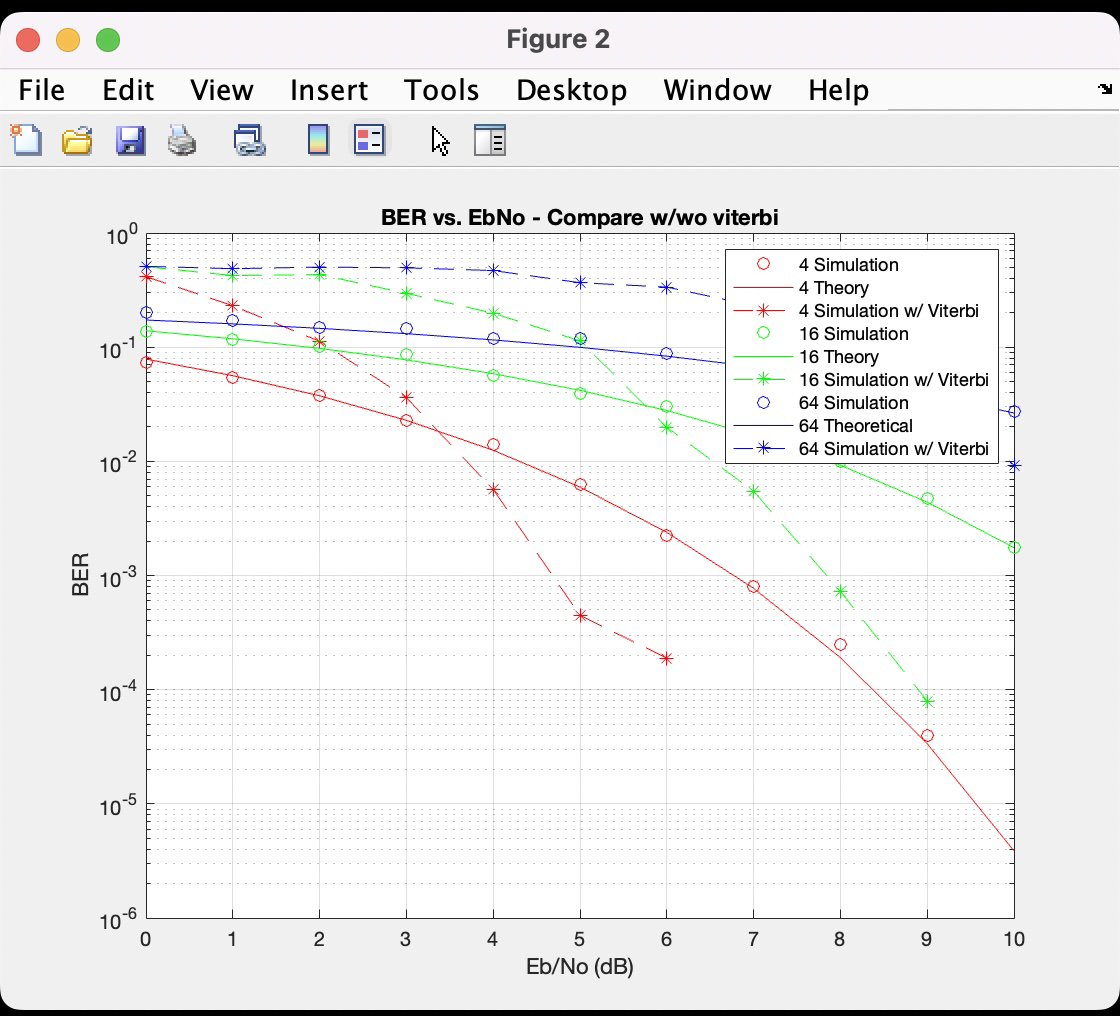
\includegraphics[width=\textwidth]{hard}
    \caption{BER with vs without Viterbi}
\end{figure}

\subsection{BER with viterbi soft decision}
\lstinputlisting[language=Matlab, caption={qam\_M\_viterbi\_soft.m}]{./matlab/qam_M_viterbi_soft.m}
\lstinputlisting[language=Matlab, caption={test\_qam\_M\_viterbi\_soft.m}]{./matlab/test_qam_M_viterbi_soft.m}
\begin{figure}[ht]
    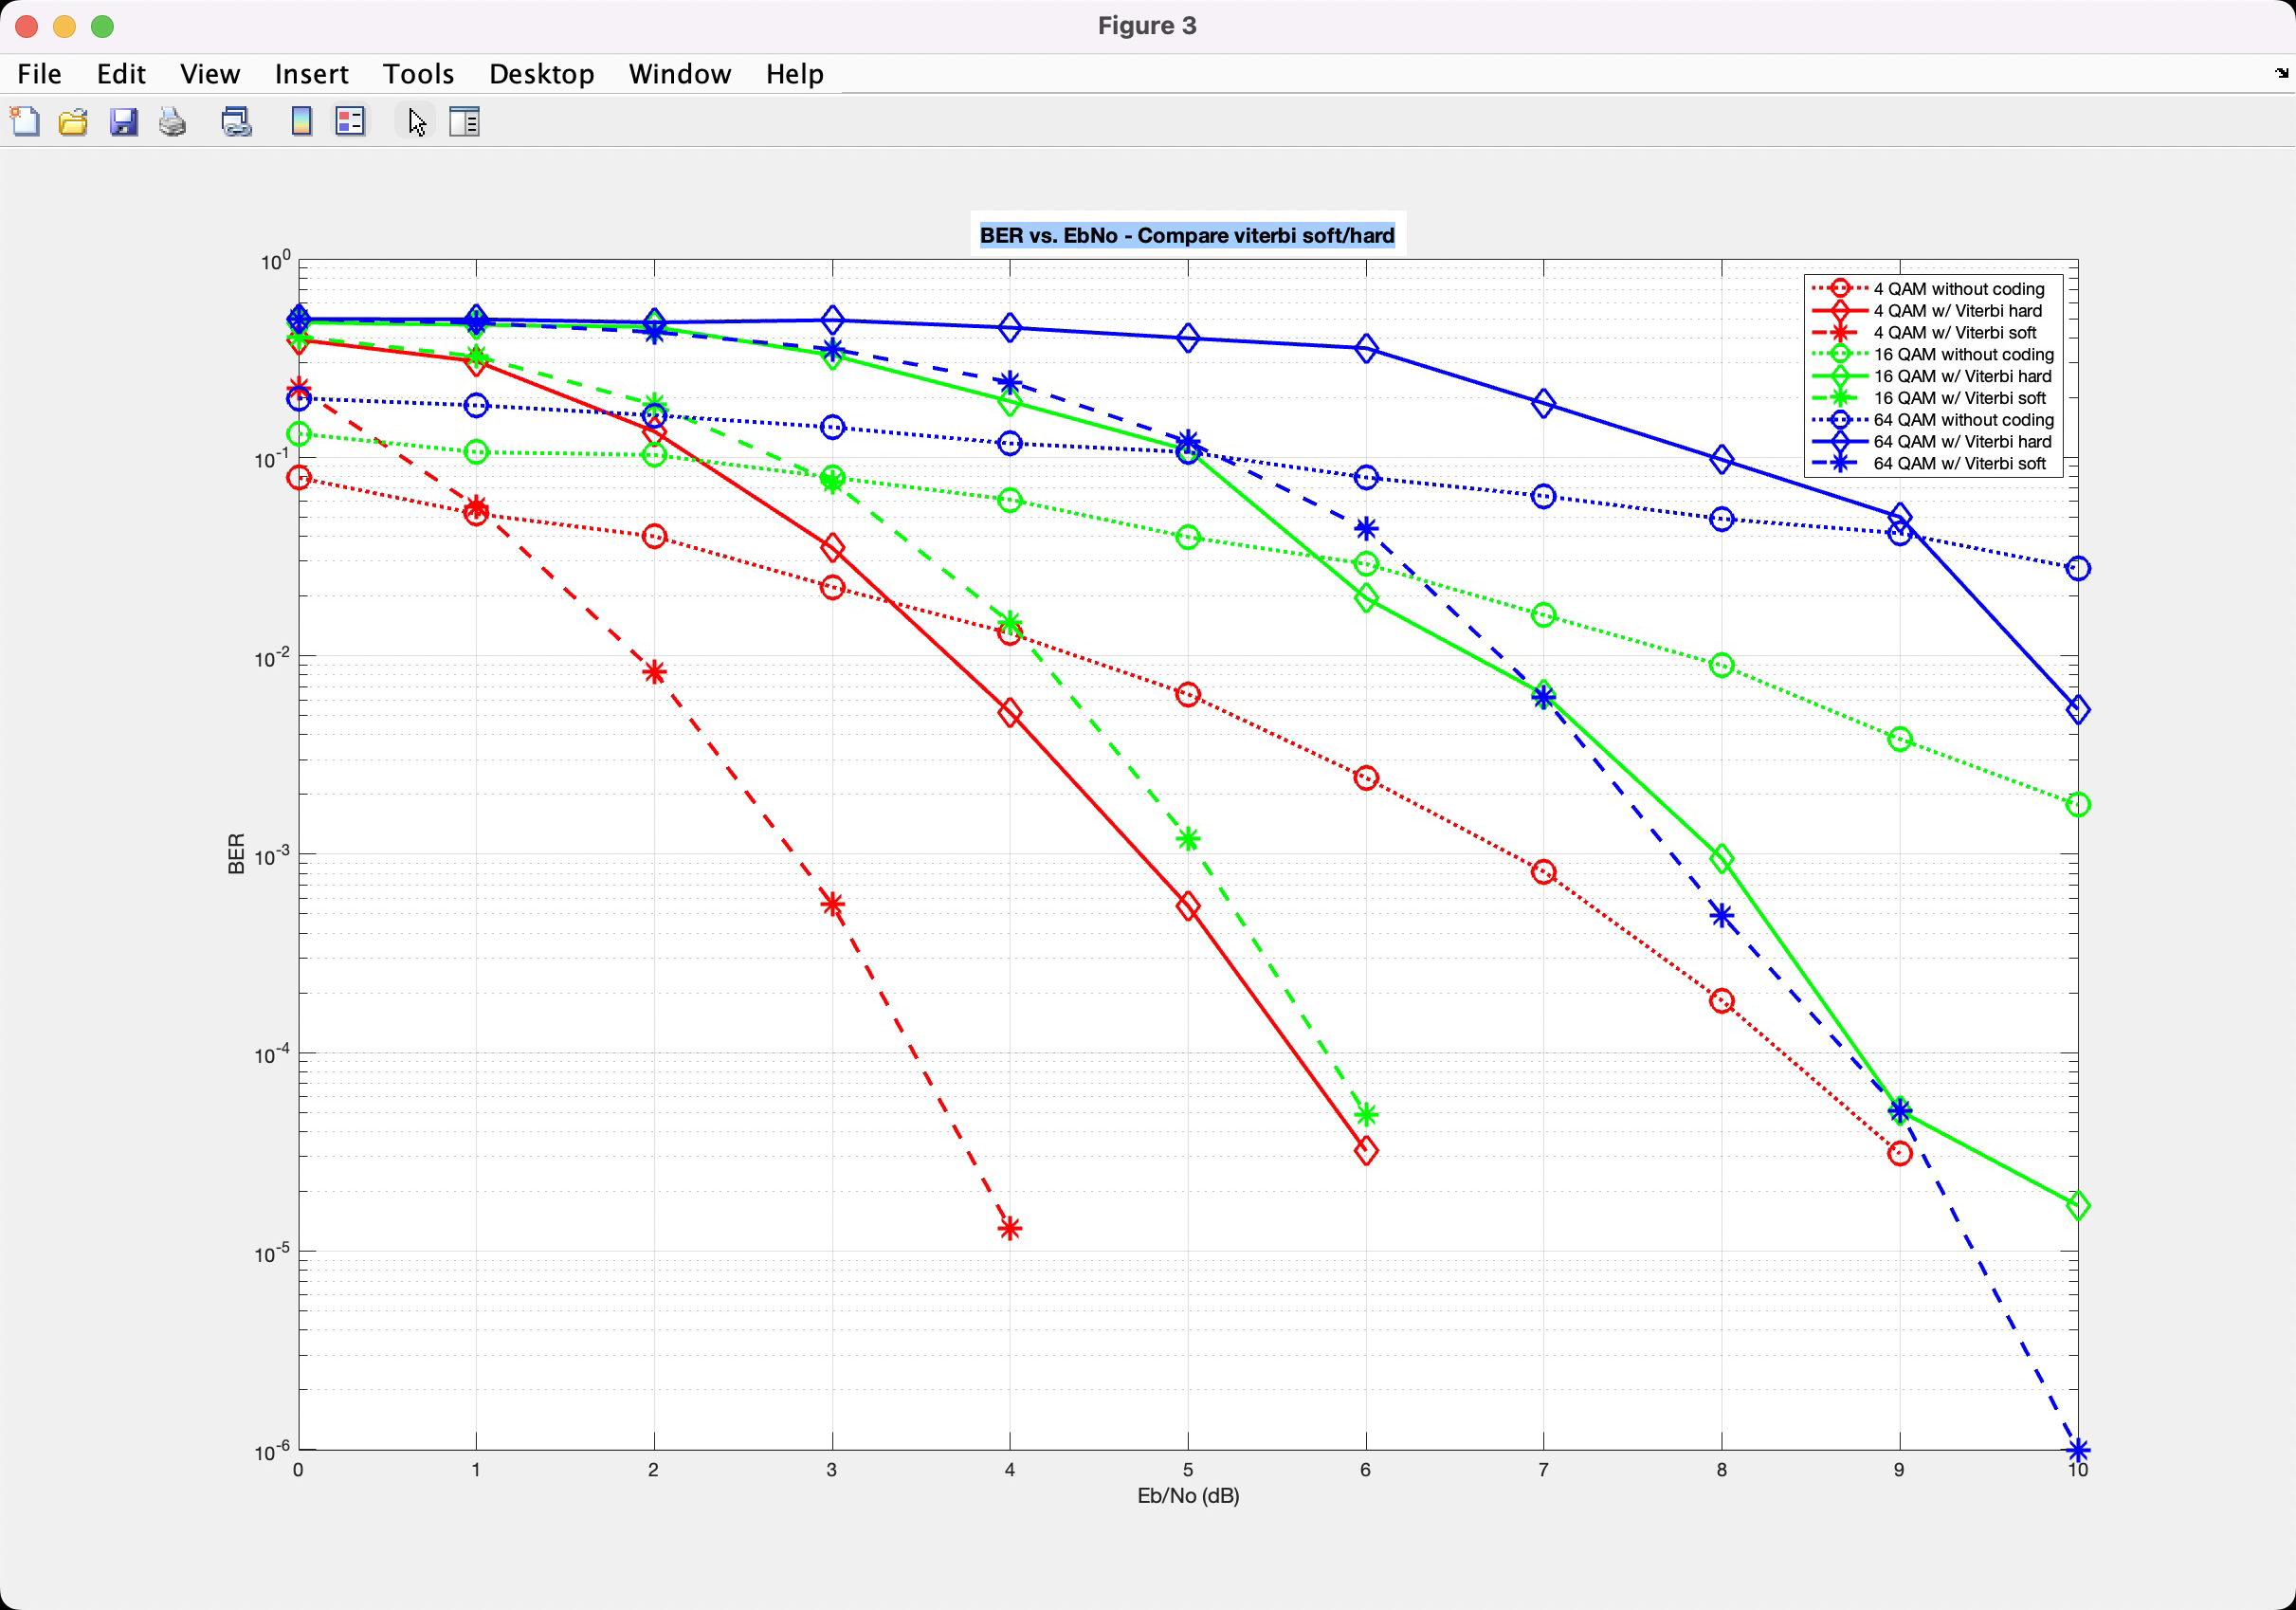
\includegraphics[width=\textwidth]{soft}
    \caption{BER Viterbi hard vs Viterbi soft}
\end{figure}

\section{Compare BER with turbo coding}
\lstinputlisting[language=Matlab, caption={qam\_M\_turbo.m}]{./matlab/qam_M_turbo.m}
\lstinputlisting[language=Matlab, caption={test\_qam\_M\_turbo.m}]{./matlab/test_qam_M_turbo.m}
\begin{figure}[ht]
    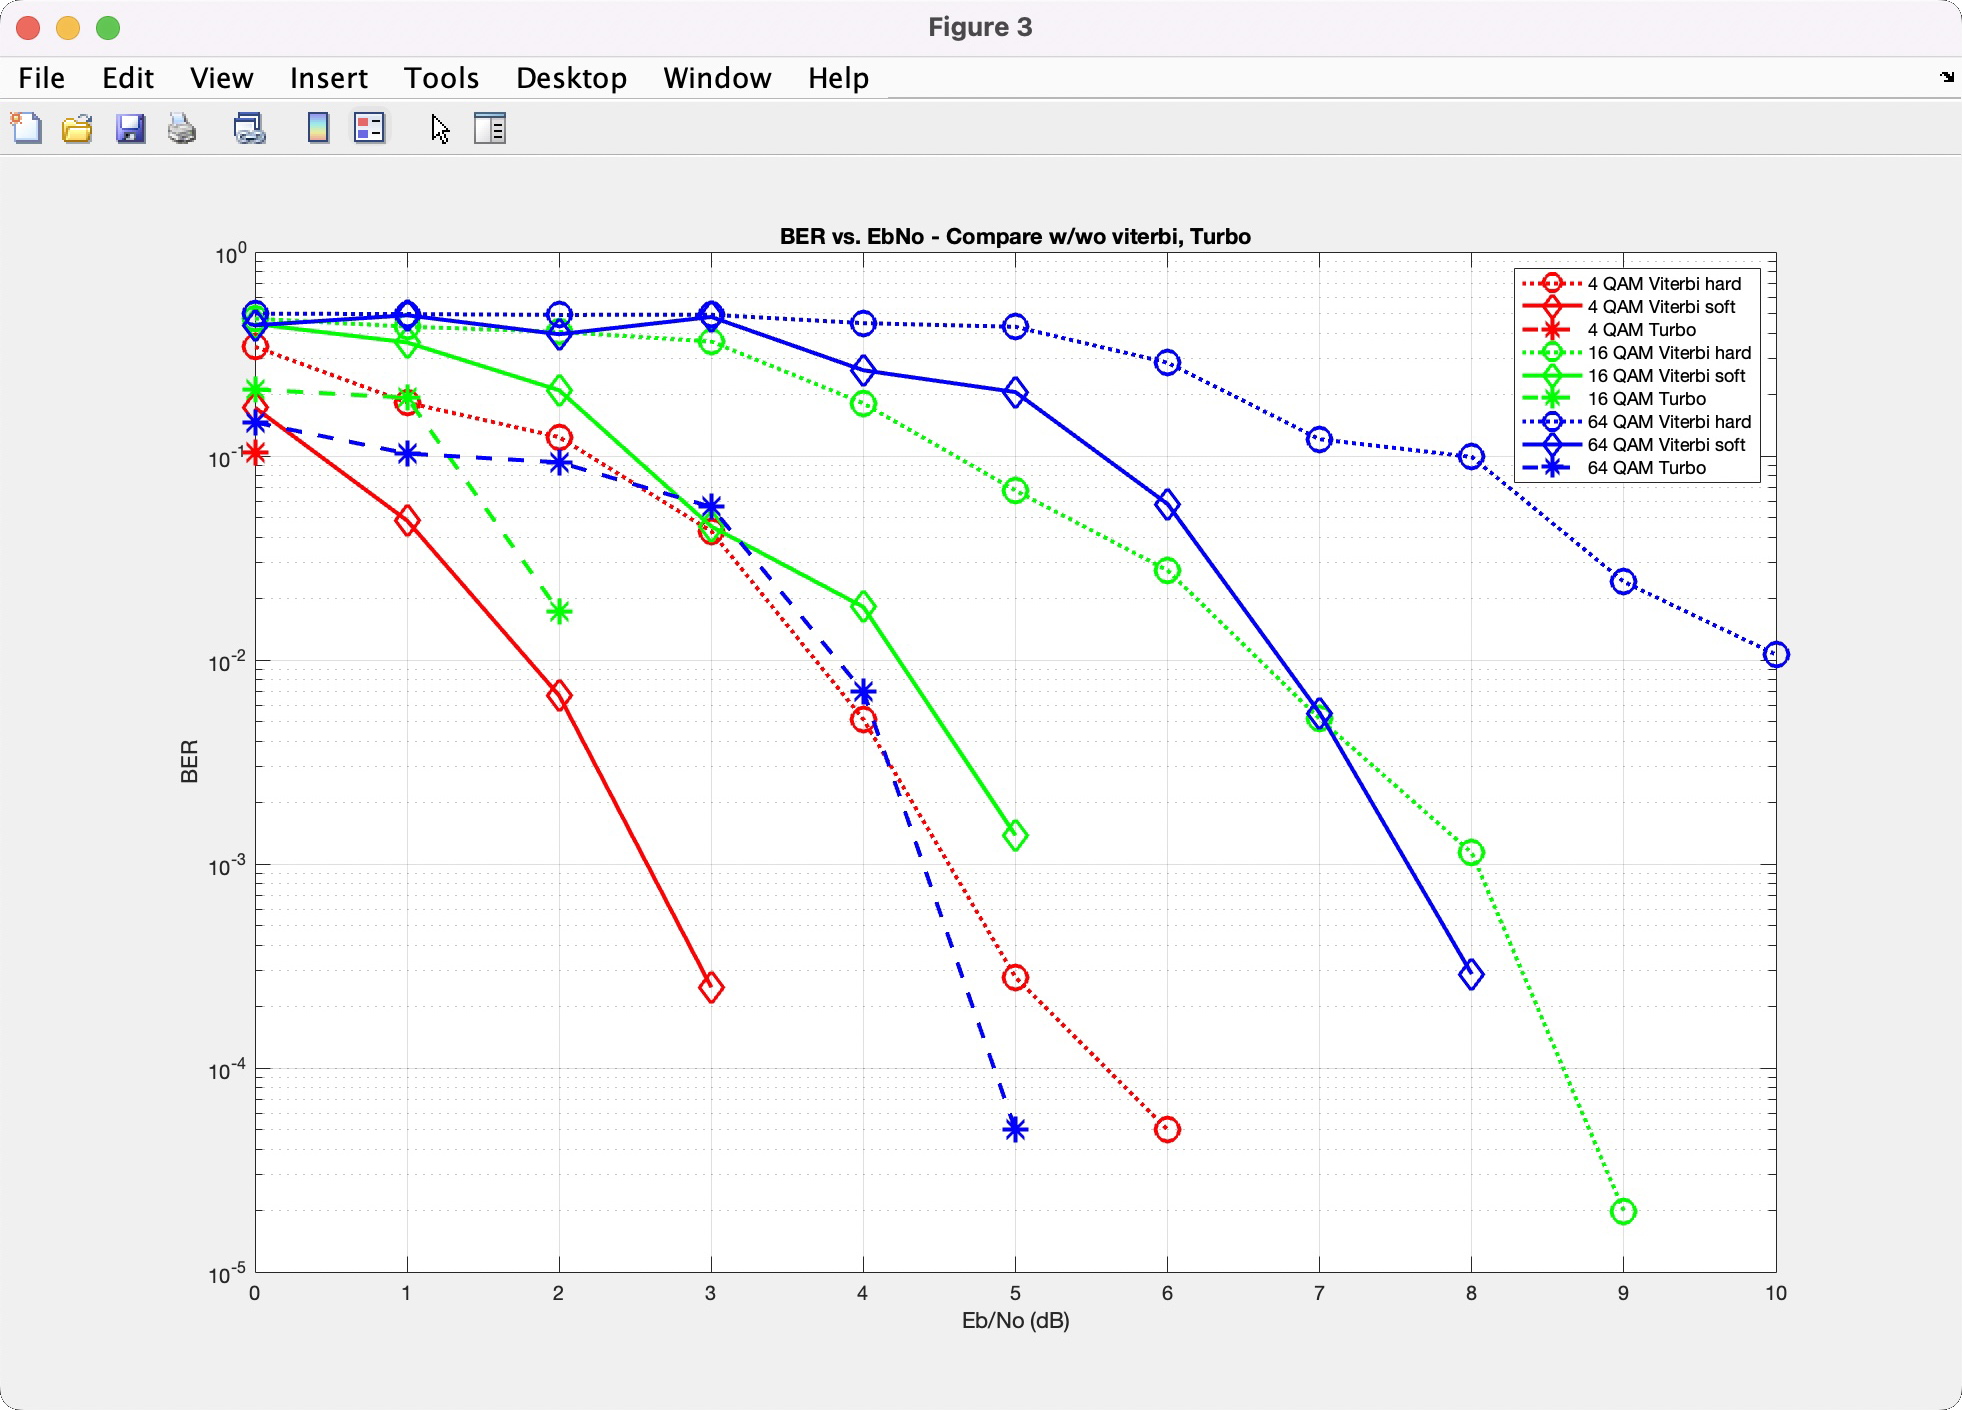
\includegraphics[width=\textwidth]{turbo}
    \caption{BER Viterbi hard vs Viterbi soft vs Turbo}
\end{figure}

\section{Compare BER with and without OFDM}
\begin{figure}[ht]
    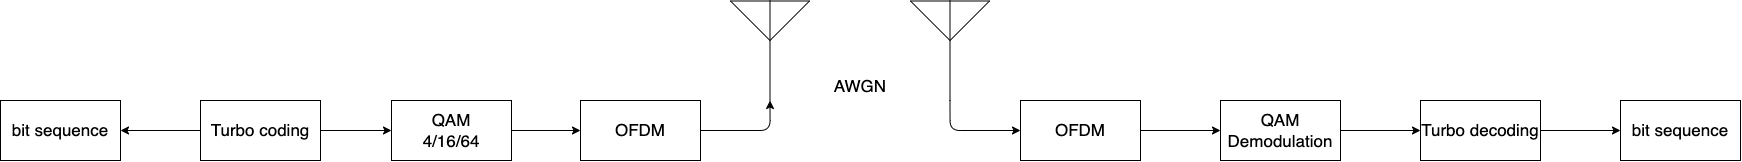
\includegraphics[width=\textwidth]{systemblock}
    \caption{System block diagram}
\end{figure}

\lstinputlisting[language=Matlab, caption={OFDMmod.m}]{./matlab/OFDMmod.m}
\lstinputlisting[language=Matlab, caption={OFDMdemod.m}]{./matlab/OFDMdemod.m}
\lstinputlisting[language=Matlab, caption={qam\_M\_turbo\_OFDM.m}]{./matlab/qam_M_turbo_OFDM.m}
\lstinputlisting[language=Matlab, caption={test\_qam\_M\_turbo\_OFDM.m}]{./matlab/test_qam_M_turbo_OFDM.m}


\begin{figure}[ht]
    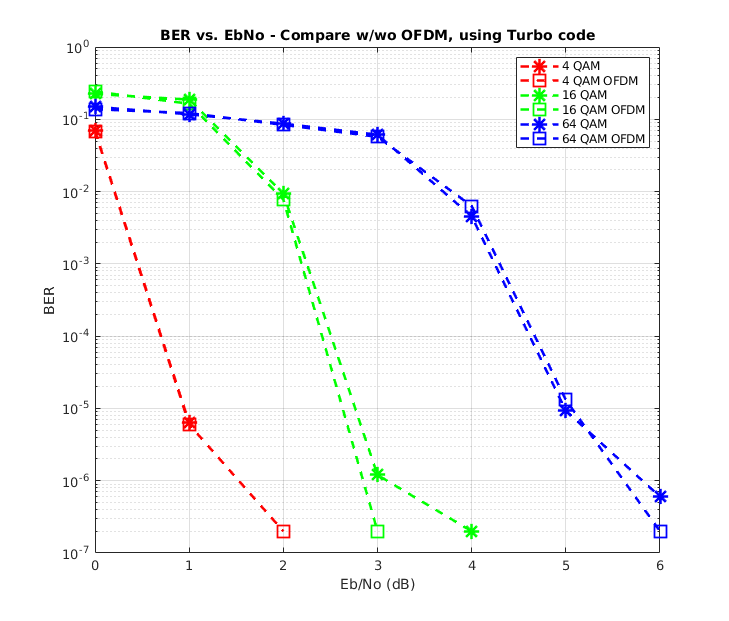
\includegraphics[width=\textwidth]{test_qam_M_turbo_OFDM_2}
    \caption{BER with vs without OFDM}
\end{figure}

\section{Source code}

The source codes and latex files are available at \url{https://github.com/ntd94/CDE204_LTE_matlab}

\end{document}